\chapter{Theory}
\label{chap:Theory}

\section{Introduction}
This chapter will provide an explanation of different types of concepts that is essential to understand before reading the rest of the thesis. It will cover various forms of software testing, multiple techniques of security testing, and other relevant information deemed necessary to understand the thesis.


\section{Software Development Lifecycle}
\acrlong{sdlc} can be defined as \textit{"structured process that enables the production of high-quality, low-cost software, in shortest possible production time. The goal of the \acrshort{sdlc} is to produce superior software that meets and exceeds all customer expectations and demands"}\cite{sdlc}.  SDLC consists of several phases that provide a framework for a software development testing and deployment. Below are the six phases that fulfill the \acrshort{sdlc}. 

  \subsection{Planning/Requirements} 
 The planning/requirements phase is the first phase of the \acrshort{sdlc}. During this phase, the project scope, objectives, and requirements are defined, as well as a plan that works as a guide, so that the software development process go as smooth as possible from the inception to completion. \cite{PlanningSDLC}
 
 \subsection{Design}
 In this phase, the development team creates high-level design of the system, including a detailed description of the architecture, components, and interfaces. This phase is considered critical because it sets the foundation for the development of the software that is being created. \cite{DesignSDLC} 
 
 \subsection{Implementation}
 It is in this phase the actual development of the software takes place. During the implementation phase, the software design is translated into code using programming languages. The implementation phase is considered quite important since this is the phase that involves the actual development of the software and the preparation of the software for deployment into the environment. \cite{ImplementationSDLC}
 
 \subsection{Testing}
 In this phase, the development team ensures that the software meets the functional, performance, and quality requirements that were decided in the earlier phases of the \acrshort{sdlc}. Here the software get tested so that any potential defects gets identified and corrected. It is in this phase the developer team ensures high quality of the software and that it meets the needs of the users. \cite{TestingSDLC}
 
\subsection{Deployment}
In the deployment phase, the process of releasing the software into the environment can be considered the main priority. In this phase the deployment team works together with the development team and other stakeholders to plan the release of the software so that it goes as smooth as possible. This also includes creating the deployment timeline, selecting a method for the deployment and defining the environment the software is being deployed into. \cite{DeploymentSDLC}

\subsection{Maintenance} 
In this phase the software has been deployed and is now being monitored to ensure that it is functioning as it was designed to do. Any refactoring and upgrades are done if needed. Monitoring the software can be done in different ways depending on how the maintenance phase has been sat up. The most common ways of monitoring however is usually through real-time reporting or ad-hoc reporting systems, which is automatically generated within the software that was created and then sent to the company that created it.\cite{MaintenanceSDLC} 

\section{Functional Testing vs Security Testing}
Software testing is a very broad area, and each test varies from according to its purpose or process - but the primary goal of software testing is to verify the quality of software systems through planned and structured testing under controlled conditions. Functional testing is emphasising on the software's behaviour and that the software is working as expected. The functional test cases are based on the requirements of the software which were specified by the stakeholder. There are several functional testing methodologies that can be conducted, such as unit testing and integration testing. White box testing and black box testing are some examples of security testing methods. This topic will be described more in section \ref{boxtesting}. 
\cite{difftesting} 

Unit testing is where small components of the code, called units, are tested. These types of tests is executed early in the SDLC, and is often done by the developers instead of testers. This is because the developers has comprehensive understanding of the code and because unit testing can help identifying bugs early, which is time-saving for the rest of the process. The purpose of these tests is to see if the code is behaving as expected by running tests on all possible components in an isolated test environment separated from other components. Integration testing looks at how the components that have already been tested in isolation perform, and confirms whether they operate as anticipated when integrated into a larger system communicating across various components. Integration testing includes both White box testing and Black box testing techniques.  \cite{unitvsintergration}

Security testing on the other hand, wants to break the software to uncover vulnerabilities. The testing aims to identify all possible weaknesses that attackers might exploit. During the testing, the testers perform the test from the attackers point of view. These kinds of test can be done manually or be done by software tools, called automated security testing tools. The goals of evaluating security functionalities is to verify if protective measures like authentication are functioning as expected. Security testing will also try to simulate attacks on the software and determine its capability to defend against them.\cite{whysectest}


\section{Box testing}
\label{boxtesting}
\subsection{Black Box Testing}
Black box testing mainly focuses on functionality and behaviour of the application without knowing the structure and processes within. One can imagine the application being a black box, not being able to see what's inside, but only focusing on the resulting output from the given input. A software will pass the black box test if input gives the expected output. \cite{blackbox}

\subsection{White Box Testing}
White box testing focuses on the application from within. In such tests, the source code and infrastructure will be looked at. The testing consist of covering paths, statements and branches, among other things. A white box tester looks for security holes by testing the code, and therefore requires to have knowledge of programming and IT. The tester looks through the code to find weaknesses such as infinite loops or data flow issues. White box testing is easier to automate than black box testing, and is often what is done for \acrlong{sast}. Despite this, it can be quite complex, and a large application with a large quantity of code can take days to test. \cite{whitebox}
\newpage

\section{Application Security Testing}
Intro

\subsection{SAST}
\acrlong{sast} is a type of software security testing tool that analysis source code of an application to identify different potentially security vulnerabilities within the code. This method of testing usually takes place during the development phase of the \acrlong{sdlc}. The primary purpose of this method is to identify and remediate security issues before the application actually is deployed. \cite{sast}

\acrshort{sast} tools scan source code for known security threats, such as \acrlong{xss}, SQL injections and buffer overflows. \acrshort{sast} tools also give warnings on any security weaknesses that may lie in the code that potentially can be exploited. After the tool has gone through the code it generates a report that contains the different vulnerabilities that it has identified, including a more in-depth description of the vulnerability and a remediation on how to fix it. 

One of the advantages with \acrshort{sast} is that it gives detailed information about the source of the vulnerability, which gives the developer a better understanding on how to fix the issue. 

There are some limitations to \acrshort{sast} tools as well. For example, it can only detect vulnerabilities that are present in the source code. This means that it cannot detect vulnerabilities that results from the interaction between different components of an application.
\begin{figure}[htp]
    \centering
    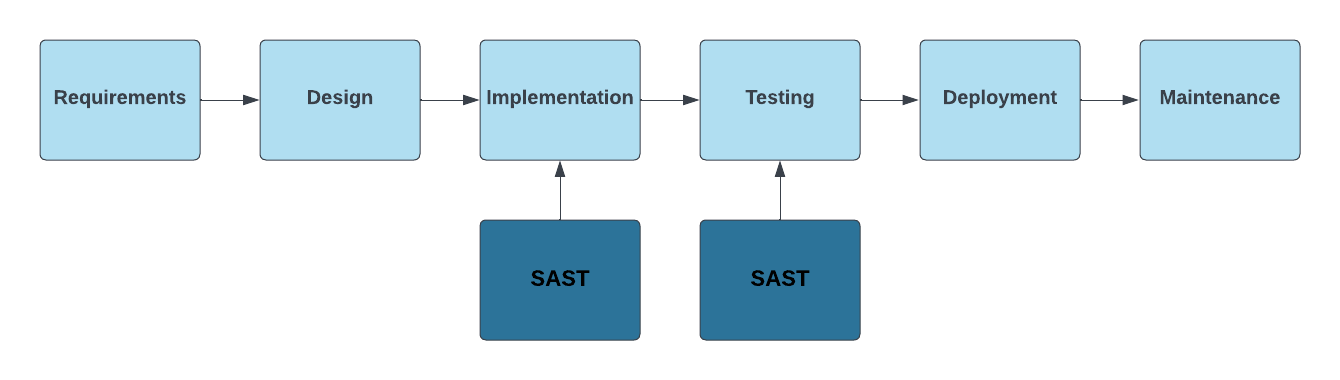
\includegraphics[width=1\columnwidth]{Images/SAST.png}
    \caption{Where to perform SAST in SDLC}
    \label{fig:my_label}
\end{figure}

\newpage
\subsection{DAST}
Compared to \acrshort{sast}, \acrlong{dast} is also a type of software security testing tool. However, what \acrshort{dast} does is that it evaluates the security of an application by performing security assessments of a running instance of the application. Unlike \acrshort{sast} which analyzes the source code of an application, \acrshort{dast} evaluates the application as its being used, this include the interaction of different components and the runtime environment. 

\acrshort{dast} simulates real-world attacks, which it does by sending malicious requests and inputs to the application it is testing and then monitoring the responses. In the end, the tool generates a report that includes the different vulnerabilities that was identified, including a more in-depth decription as well as a remedation on how to fix the issue. \cite{dast}

An advantage with \acrshort{dast} is that it can identify security issues that is not detectable through \acrshort{sast}, this can for example be interactions between different components. Another advantage is that with \acrshort{dast}, it can identify different vulnerabilities that gets triggered, for example when the application is under heavy load or when are specific inputs received.

However, there are some limitations with \acrshort{dast} as well, one being that it can only detect vulnerabilities that are present in the deployed version of the application and cannot give in-depth description on vulnerabilities that lie in the source code.

\begin{figure}[htp]
    \centering
    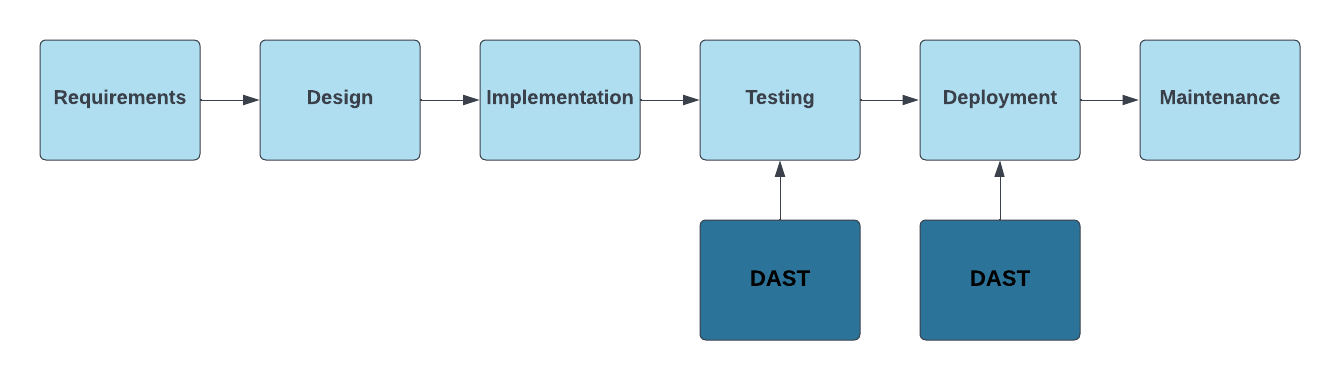
\includegraphics[width=1\columnwidth]{Images/DAST.png}
    \caption{Where to perform DAST in SDLC} 
    \label{fig:my_label}
\end{figure}

\newpage

\subsection{SCA}
\acrlong{sca} is, compared to the others, also a type of software security testing tool. What \acrshort{sca} does is that it analyzes the dependencies of a software application to identify and manage potential security risks. The main objective of the \acrshort{sca} is to identify third-party components that may contain security vulnerabilities. \cite{sca}

 \acrshort{sca} scans the application's code to identify all of its dependencies, including the different versions of the components used. It then cross-references these dependencies to different databases that include known vulnerabilities. It then generate a report containing any potential risk. In comparison to the others, the report also includes an in-depth description of the vulnerability as well as a recommendation to update the components to newer versions or replacing these. 

An advantage with \acrshort{sca} is that it can quickly identify risks that may be introduced from third-party components. It is rather common that modern applications relies on a large number of  different dependencies, which therefore make \acrshort{sca} useful. It can provide a comprehensive view of the security risks associated with an application and help developers make informed decisions about the security and their applications. 

However, it is important to remember that \acrshort{sca} does not always have access to updated information, and may give some false-positives about vulnerabilities that doesn't necessary exist anymore. 


\begin{figure}[htp]
    \centering
    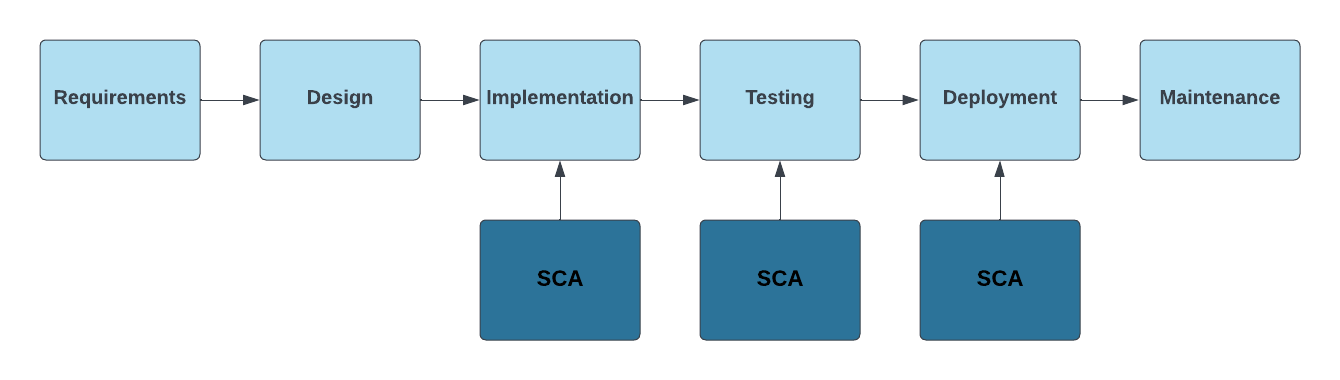
\includegraphics[width=1\columnwidth]{Images/SCA.png}
    \caption{Where to perform SCA in SDLC} 
    \label{fig:my_label}
\end{figure}

\newpage
\subsection{Comparison of SAST, DAST and SCA}
The table below show the similarities between SAST, DAST and SCA. A combination of these can in cases increase the security drastically. 
\begin{figure}[htp]
    \centering
    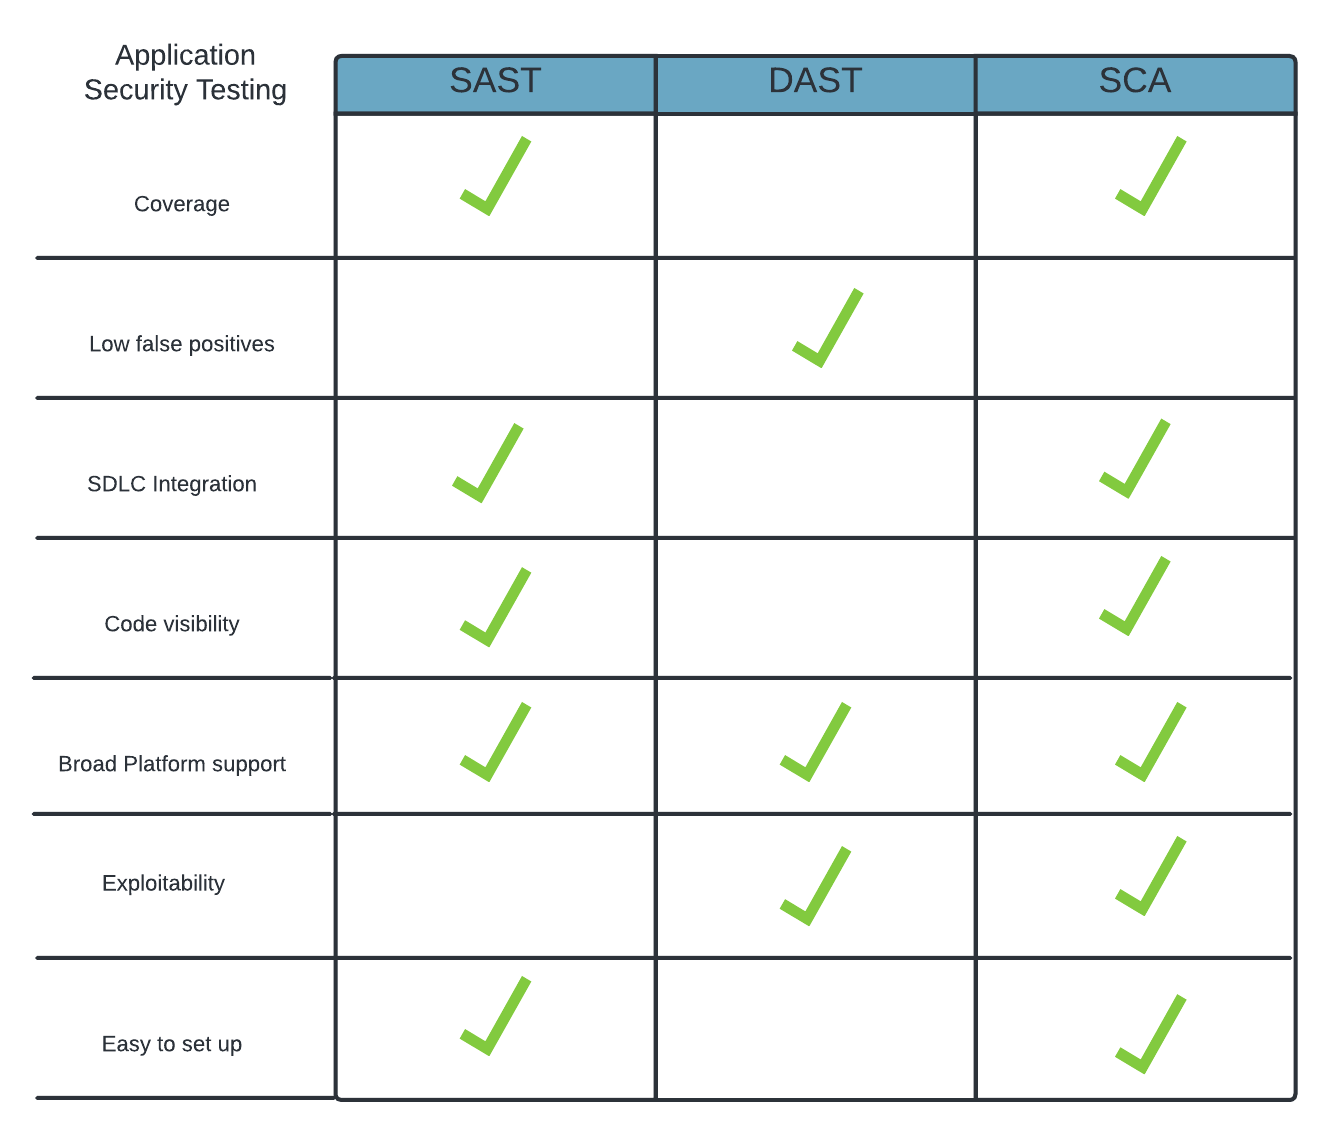
\includegraphics[width=1\columnwidth]{Images/SCA vs DAST vs SAST.png}
    \caption{Comparison of SCA, DAST and SAST}Adapted from: \cite{Comparison}
    \label{fig:my_label}
\end{figure}



\newpage
\section{The Significance of Software Security Testing}
Security testing plays a critical role in the \acrlong{sdlc}, as it is employed to identify potential security vulnerabilities in the system and prevent real-world attacks. It is a process where the security of the system is evaluated and identifies the system's possible security weaknesses and risks of vulnerability.\cite{whysectest}

In 2022, the cost of a data breach were estimated to be USD 4,35 million\cite{databreach}, but the expenses to prevent breaches like this is significantly lower. To repair a vulnerability in the design phase costs an average of USD 500\cite{fixvulnerability}. Starting software testing early in the SDLC results in reduced costs and time-saving. 

As mentioned in sections 2.3, there are various types of testing that should be executed on an application, including testing of both the written code and the libraries that are integrated and being used. It is crucial to test libraries because they can contain various types of vulnerabilities, especially if they are open source. This is because open-source code is open to common vulnerabilities, which can expose the application to malware injections, distributed denial-of-service (DDoS) attacks, and exposure of sensitive data. \cite{testlibaries}


\section{Vulnerability Risk Rating}
Discovered vulnerabilities can be rated by standardized systems like CVSS, CVE, CWE and OWASP Risk Rating Methodology. 
\subsection{Common Vulnerability Scoring System (CVSS)}
\acrlong{cvss}, know as \acrshort{cvss}, is \textit{"an Security Content Automation Protocol (SCAP) specification for communicating the characteristics of vulnerabilities and measuring their relative severity"}\cite{nistCVSS}. The system is used to give vulnerabilities a numeric score based on it´s severity. The scores can be translated into low, medium, high and critical to assist organizations to evaluate and rank their vulnerabilities. CVSS is currently at version 3.1. \cite{CVSS}
\begin{figure}[htp]
    \centering
    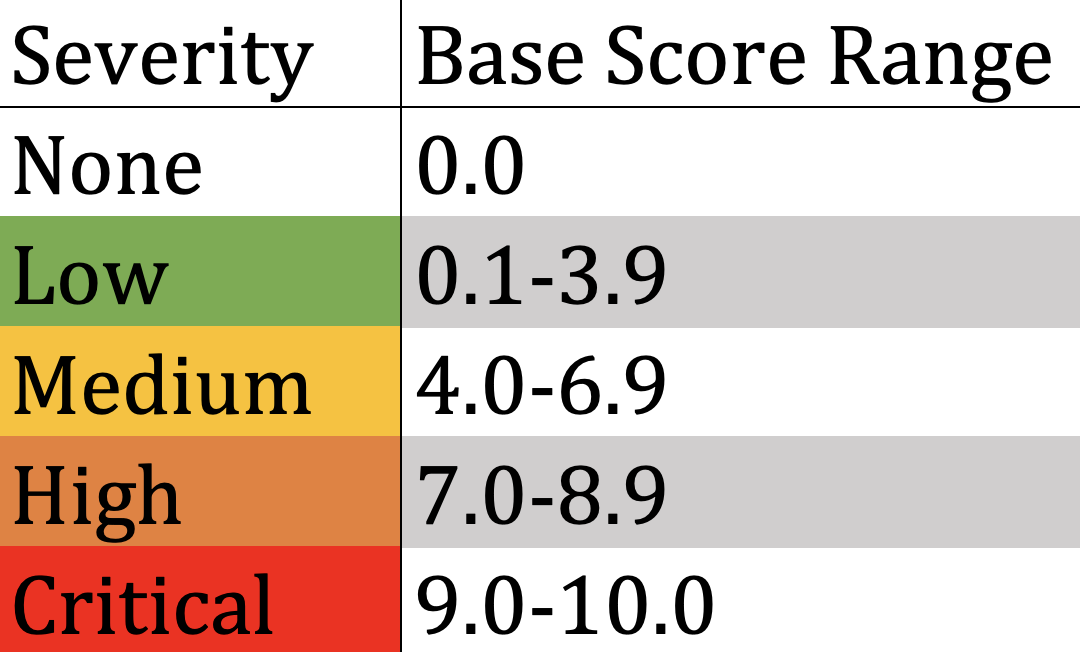
\includegraphics[scale=0.3]{Images/CVSS.png}
    \caption{CVSS v3 Ratings} Adapted from:\cite{cvssrating}
    \label{fig:my_label}
\end{figure}

\subsection{Common Vulnerabilities and Exposures (CVE)}
\acrlong{cve}, known as \acrshort{cve}, is, according to their website,\textit{"a list of records each containing an identification number, a description, and at least one public reference for publicly known cybersecurity vulnerabilities"}\cite{CVE}. The CVE program's mission is to determine, describe, and categorize cybersecurity vulnerabilities that have been made public. All discovered vulnerabilities will be put into records and sent to NVD.\cite{CVE}

\subsection{Common Weakness Enumeration (CWE)}
\acrlong{cwe}, know as \acrshort{cwe}, is \textit{"a community-developed list of common software and hardware weakness types that have security ramifications"}\cite{CWE}. It was established to serve as a consistent benchmark for security solutions that address vulnerabilities, and as a baseline for identifying, mitigating, and preventing weaknesses. CWE's goals is to provide instructions for those who have control over and maintain source code to stop the vulnerabilities at the source.\cite{CWE} 

\subsection{OWASP Risk Rating Methodology}
OWASP Risk Rating Methodology is an approach which is regularly used in the industry, due to its focus on prioritizing security risks associated with software applications. It contains a formula  that calculates a risk score for each vulnerability based on two factors: likelihood and impact. There are multiple factors which make up the both likelihood and impact. 

Factors that together compose the estimation of likelihood are separated into different groups which is related to threat actor and the vulnerability. The set of factors related to the threat actor are skill level, motive, opportunity, and size. The set of factors related to the vulnerability is ease of discovery, ease of exploit, awareness, intrusion detection. Each factor will have different options, where each option will receive a likelihood rating from 0-9. 

Factors that together compose the estimation of impact are divided into technical impact and business impact. Technical impact is broken down into confidentiality, integrity, availability, and accountability. Further, business impact is divided into financial damage, reputation damage, non-compliance and privacy violation. All of the factors will, like the factors of likelihood, receive a impact rating from 0-9. 

Combining the estimates of likelihood and impact factors produces an overall severity level of the risk, which can be classified as low, medium, or high (as shown in figure 2.5) in order to determine its severity. These levels can be further combined to determine the final severity of the risk, as illustrated in figure 2.6. 

\begin{figure}[htp]
    \centering
    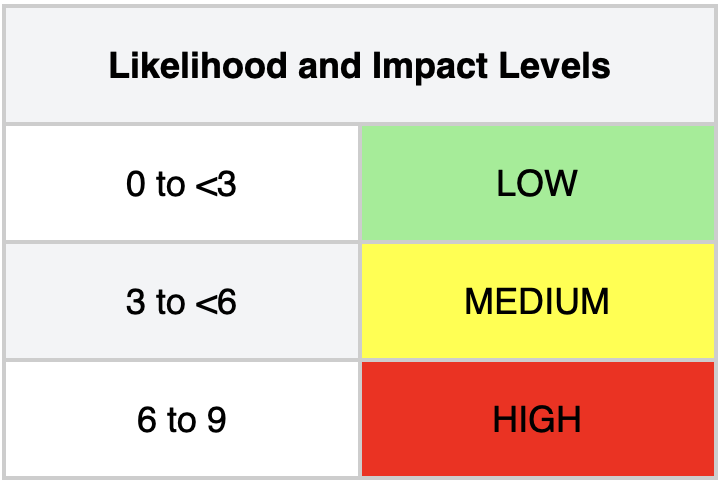
\includegraphics[scale=0.5]{Images/OWASP-likelihood.png}
    \caption{The likelihood and impact levels}
    \label{fig:my_label}
\end{figure}

\begin{figure}[htp]
    \centering
    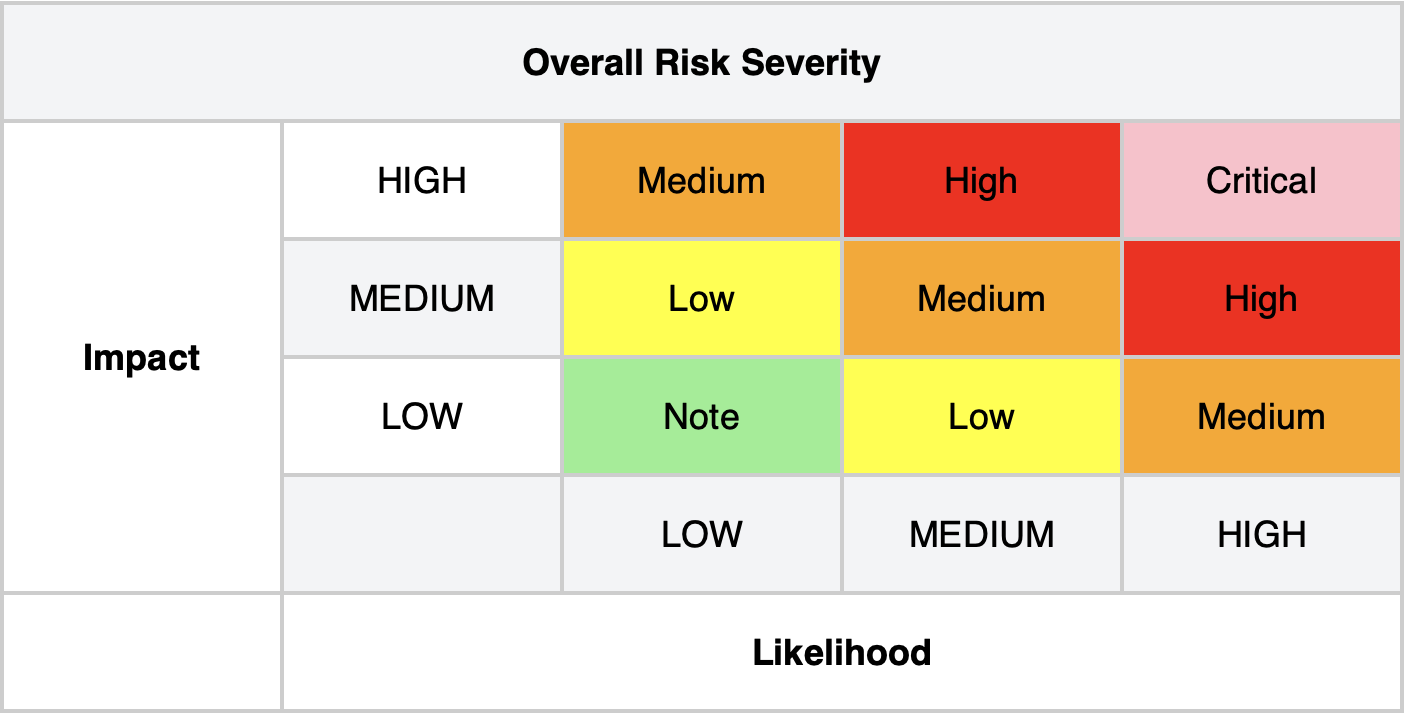
\includegraphics[scale=0.4]{Images/OWASP-severity.png}
    \caption{Severity level based on impact and likelihood}
    \label{fig:my_label}
\end{figure}
\section{placeholder}